%!TEX root = thesis.tex
\chapter{Paralleler Algorithmus} % (fold)
\label{cha:paralleler_algorithmus}

\section{Vorüberlegungen} % (fold)
\label{sec:vor_berlegungen}
Eine einzelne Instanz der Breitensuche ist relativ schwer und nur unter recht hohem Synchronisationsaufwand nebenläufig lösbar. Das liegt daran, dass keine unabhängigen Ausführungsstränge definierbar sind. Überlegungen, etwa jedem Prozess eine starke Zusammenhangskomponente des Graphen zur Berechnung zu geben, scheitern bereits daran, dass allein die Laufzeit der Graphpartitionierung schon mindestens so lang wie die der Breitensuche ist. Um grundsätzlich die BFS-Distanz eines Knotens zu setzen, muss die Distanz des Vorgängers bekannt sein. Wegen der Forderung im folgendem Absatz liegt diese aber im Allgemeinen nicht im eigenen Speicher vor. Deswegen muss für jede Iteration der BFS in irgendeiner Weise eine Kommunikation stattfinden.

Weiterhin muss zu jedem Knoten die aktuelle BFS-Distanz gespeichert werden, was global O(n) Speicheraufwand bedeutet. Um bei sehr großen Graphen nicht extern arbeiten zu müssen, wird deswegen gefordert, bei p Prozessen mit O(n/p) + O(1) Speicherbedarf je Prozess auszukommen. Für eine bessere Anschaulichkeit werden in den folgenden theoretischen Überlegungen zunächst Adjazenzmatrizen als Graphrepräsentation verwendet, auch wenn reale Graphen oft eher dünn besetzt sind und Adjazenzmatrizen deswegen eher ungeeignet sind. Dabei sei $A(i,j) = true$, wenn eine gerichtete Kante von i nach j existiert. Im folgenden werden die zwei grundlegenden Konzepte der Breitensuche \cite{Buluc:2011} vorgestellt. Der Name 1D bzw. 2D Partitionierung bezieht sich dabei auf die Aufteilung der Daten auf Places.
% section vor_berlegungen (end)

\section{Datenstrukturen für Graphen} % (fold)
\label{sec:datenstrukturen_f_r_graphen}
Im Laufe dieser Arbeit wurde eine serielle Version der Breitensuche implementiert, um unter anderem verschiedene Datenstrukturen für Graphen zu testen. Implementiert wurde die Breitensuche immer nach dem Schema von Algorithmus \ref{alg:sequential_bfs} auf Seite \pageref{alg:sequential_bfs}. Die verschiedenen Implementierungen unterscheiden sich nur in der Weise, wie über die adjazenten Kanten iteriert wird, da nur an dieser Stelle die Graphrepräsentation eine Rolle spielt. Die implementierten Datenstrukturen sind:
\begin{description}
	\item [Adjazenzmatrizen] Adjazenzmatrizen haben unabhängig von der Dichte eines Graphen einen Speicherbedarf von $\Theta(n^2)$. Die Iteration über alle Kanten, die adjazent zu einem Knoten sind, benötigt immer $\Theta(n)$ Schritte, unabhängig davon, wie viele Kanten wirklich adjazent sind. Diese unteren Schranken machen Adjazenzmatrizen für solche Graphen geeignet, deren Ausgangsgrad in $\Theta(n)$ liegt. Pro Eintrag in der Matrix reicht 1 Bit speicher aus.
	\item [Adjazenzlisten] Die Implementierung verwendet ein Array, das für jeden Knoten eine Liste aller ausgehenden Kanten enthält. Als Listen wurden Arraylisten eingesetzt. Der Aufwand zur Iteration über alle Kanten eines Knoten ist bei Adjazenzlisten linear zu der Anzahl der Kanten. Im Vergleich zu den Adjazenzarrays muss hier für jede Kante ine ganze Zahl gespeichert werden. Deswegen brauch diese Datenstruktur bei dichten Graphen mehr Speicher.
	\item [Adjazenzarrays] Die Implementierung von Adjazanzarrays entspricht der aus \cite{SWB-283374373}. Es werden zwei Arrays benötigt, eines der Länge n+1, genannt V und eines der Länge m, genannt E. Um alle außgehenden Kanten eines Knoten i zu finden, muss über das Array E von der Stelle V[i] bis V[i+1] iteriert werden. Es wird V[i+1] = m+1 gesetzt um zu garantiert, dass der Eintrag in V an der Stelle i+1 für alle gültigen i existiert. Im Grunde entspricht das einer Optimierung der Adjazenzlisten, die möglich ist, weil keine neuen Kanten im Laufe des Algorithmus hinzukommen.
\end{description}

Die durchgeführten Tests zeigten die zu erwartenden Ergebnisse. Adjazenzlisten mittels Arrayliste oder mittels Adjazenzarrays erreichen meistens eine sehr viel höhere Performance als Matrizen. Wie zu erwarten nimmt der Vorsprung der Listen gegenüber Matrizen ab, umso dichter die Graphen sind. Einen Unterschied zwischen der Performance von Adjazenzarrays und Adjazenzlisten konnte nicht festgestellt werden, weswegen für die weitere Arbeit ausschließlich Adjazenzlisten verwendet wurden. Diese haben weiterhin den Vorteil, dass sie für jeden Knoten eine eigene Liste verwenden. Bei der Partitionierung auf mehrere Places vereinfacht das die Implementierung.

% TODO: Ergebnisse hier einfügen oder drauf verweisen

% section datenstrukturen_f_r_graphen (end)

\section{1D Partitionierung} % (fold)
\label{sec:1d_partitionierung}
Bei der 1D Paritionierung wird die Adjazenzmatrix entlang genau einer Dimension aufgeteilt. Die Aufteilung erfolgt derart, dass jeder Knoten genau einem Place gehört und jeder Place möglichst gleich viele Knoten besitzt. Es ist wichtig, dass jeder Place sehr schnell (in O(1)) herausfinden kann, welchem Place ein bestimmter Knoten gehört. Um dies zu erreichen, sollte es einen arithmetischen Zusammenhang von Knoten k zu seinem besitzenden Place p geben. Die nötige Arithmetik wird durch eine Distribution abstrahiert. Außerdem wird definiert, dass alle Kanten, die von Knoten k ausgehen, demselben Place gehören, wie Knoten k. Diese Partitionierung entspricht einer horizontalen Zerschneidung der Matrix.

\begin{center}
$\left( \begin{array}{c}
	\dots \\ Daten\;von\;Prozess\;1 \\	\hline
	\dots \\ Daten\;von\;Prozess\;2 \\	\hline
	\dots \\	\hline
	\dots \\ Daten\;von\;Prozess\;p \\
\end{array} \right)$
\end{center}

Diesem Muster folgend wird auch das BFS-Distanz Array partitioniert. Der Place, dem ein Knoten gehört, ist dem entsprechend der einzige, der die BFS-Distanz dieses Knotens kennt. Damit wissen auch nur alle Aktivities auf diesem Place, ob der Knoten bereits erreicht wurde oder nicht. Sehr abstrakt kann der verwendete Algorithmus wie in \ref{alg:1d_bfs_abstract} beschrieben werden. Dabei ist zu beachten, dass der Pseudocode an X10 angelehnt ist. Die erste Zeile wird nur auf dem ersten Place ausgeführt. Die anderen Places werden erst ab Zeile 2 aktiviert. Entsprechend der X10 Nomenklatur wertet $dist(k)$ zu dem Place aus, dem der Knoten k gehört.

\begin{algorithm}
	\caption{1D-partitionierte Breitensuche}
	\label{alg:1d_bfs_abstract}
	\begin{algorithmic}[1]
		\State {Startknoten: s, Kantenanzahl: n, Anzahl Places: p}
		\State bfsDistance : DistArray of size n \Comment{Mit $\infty$ initialisiert, 0 an Stelle s}
		\For{each place, do async on place}
			\State{current : List<Nodes>}(s) \Comment{Lokale Liste pro Place}
			\While{$\sum\limits_{i=0}^{p-1} \#current_i > 0$}
				\State{//Phase 1:}
				\For{$ u \in current$}
					\For{each neighbor v of u}
						\State{put u in the sendbuffer for place dist(u)}
					\EndFor
				\EndFor
				\State{//Phase 2:}

				\State{Send sendbuffer to corresponding place}
				\State{$barriere$}
				\State{//Phase 3:}
				\For{u in receivebuffer}
					\If{$bfsDistance(u) == \infty$}
						\State{Update bfsDistance(u)}
						\State{Put u in current}
					\EndIf
				\EndFor
			\EndWhile
		\EndFor
	\end{algorithmic}
\end{algorithm}

Es gibt auf jedem Place zunächst genau eine Aktivität. Zur Initialisierung erstellt sie auf ihrem jeweiligen Place lokal eine Liste aus aktiven Knoten (Zeile 4). Die Liste wird auf allen Places leer initialisiert, außer auf dem Place, dem der Startknoten gehört. Dort wird der Startknoten in die Liste eingefügt. Der Algorithmus kann in 3 Phasen aufgeteilt werden, die jeweils in sich lokal auf einem Place ablaufen. Es wird solange über die 3 Phasen iteriert, bis auf allen Places die Liste der aktiven Knoten leer ist.

\subsection{Phase 1: Adjazente Knoten sortieren} % (fold)
\label{sub:phase_1}
In Phase 1 wird auf jedem Place für sich über die Liste der aktiven Knoten iteriert. Nach Voraussetzung stehen in der Liste nur Knoten, die dem jeweiligen Prozess selbst gehören, deswegen kennt der Prozess auch alle ausgehenden Kanten. Zu jeder Kante muss der Algorithmus nun herausfinden, welchem Place der Zielknoten gehört und den Knoten in einen entsprechenden Sendepuffer einordnen. Am Ende dieser Phase ist die Liste der aktiven Knoten leer.
% subsection phase_1 (end)

\subsection{Phase 2: Kommunikation} % (fold)
\label{sub:parallel_phase_2}
Phase 2 ist die Kommunikationsphase. Von jedem Place werden die Sendepuffer an die jeweiligen Empfänger geschickt. Hier ist zu bemerken, dass jeder Place einen Empfangspuffer für jeden anderen Place bereithalten muss. Wenn es p Places gibt, gibt es also global ($p^2$) Empfangspuffer, je p davon liegen auf einem Place. Wenn es nur einen geteilten Empfangspuffer für pro Place gäbe, wäre hier weitere Synchronisation notwendig. Es ist also eine Abwägung zwischen Speicherplatz und Rechenzeit. Das Mehr an Speicheraufwand von p Puffern ist vernachlässigbar klein, da ein leere Liste kaum Platz benötigt. In X10 wird der Empfangspuffer als DistArray implementiert, der pro Place ein Array von Empfangspuffern hält. Der Sendevorgang wurde als asynchrone for-Schleife über alle Places implementiert. Der Place-Wechsel mittels \textit{at\{place\}} wird nur ausgeführt, wenn es tatsächlich Daten zu senden gibt. Nach dieser Phase wird eine globale Barriere benötigt, da im nächsten Schritt die Empfangspuffer ausgewertet werden, die in dieser Phase erst geschrieben werden.
% subsection phase_2 (end)

\subsection{Phase 3: BFS-Distanz aktualisieren} % (fold)
\label{sub:phase_3}
Jeder Prozess hat eine Menge von Empfangspuffern. Alle Knoten, die in den Puffern stehen, gehören nach korrektem Ablauf von Phase 2 dem Prozess selbst. Außerdem gilt für alle Knoten, dass sie von den Knoten der letzten Iteration aus erreichbar sind. Phase 3 entspricht dem Aktualisieren der klassischen Breitensuche. Es wird über alle Knoten in allen Empfangspuffern iteriert. Wenn die BFS-Distanz noch auf $\infty$ steht, wird sie auf die Nummer der aktuellen Iteration gesetzt und der Knoten der Liste der aktiven Knoten hinzugefügt, wenn die BFS-Distanz kleiner als $\infty$ ist, wird der Knoten ignoriert und verworfen. 
Um die BFS-Distanz auf die Nummer der aktuellen Iteration zu setzen, muss die Anzahl der Iterationen mitgezählt werden. Durch die Synchronisation kann das lokal auf jedem Place passieren. Ein einfacher Schleifenzähler reicht aus.
% subsection phase_3 (end)


\subsection{Place-lokale Parallelität} % (fold)
\label{sub:place_lokale_parallelit_t}
Auch wenn das eigentliche Thema dieser Arbeit nicht die Parallelisierung auf Shared-Memory Architekturen ist, soll hier kurz beschrieben werden, wie die einzelnen Phasen auf einem Place nebenläufig implementiert werden können, falls mehr als ein Kern auf einem Place zur Verfügung steht.
\begin{description}
	\item[Phase 1] Hier ist einfach Schleifenparallelität möglich. Dabei muss beachtet werden, dass Zugriffe auf die Sendepuffer synchron passieren. In X10 lässt sich das einfach mit einem \textit{finish}, einem \textit{async} und einem \textit{atomic} für den Pufferzugriff bewerkstelligen. Im Allgemeinen kann auch für jeden Ausführungsfaden ein eigenes Set an Sendepuffern erstellt werden, die dann vor dem Versenden zusammengeführt werden. Diese Methode widerstrebt allerdings der Philosophie der impliziten Parallelisierung durch X10. Mehr zu den Problemen dieser Phase ist in Abschnitt \ref{sub:optimierungen} zu finden.	
	\item[Phase 2] Da Phase 2 nur aus dem Versenden der Puffer besteht, muss offensichtlich nur sichergestellt werden, dass das Versenden asynchron passiert. Da eine Synchronisationsbarriere nach dieser Phase nötig ist, müssen alle Sendevorgänge vollständig abgeschlossen sein, bevor die Barriere betreten werden darf.
	\item[Phase 3] In Phase 3 werden die Empfangspuffer ausgewertet. Auch hier ist wieder einfache Schleifenparallelität, wie sie X10 anbietet, möglich. Da die Liste der aktiven Knoten für die nächste Iteration geschrieben wird, ist wiederum ein synchronisierter Zugriff notwendig. Es gibt auch hier wie in Phase 1 die Möglichkeit, einzelne Puffer pro Ausführungsfaden zu benutzen, was hier aber nicht getan wurde.
\end{description}
% subsection place_lokale_parallelit_t (end)

\subsection{Optimierungen} % (fold)
\label{sub:optimierungen}

\subsubsection{Duplikate in Sendepuffern} % (fold)
\label{sub:duplikate_in_sendepuffern}
Es ist sehr wahrscheinlich, dass ein Knoten in einer Iteration gleichzeitig über mehrere Kanten erreicht wird. Um so dichter der betrachtete Graph ist, desto wahrscheinlicher wird der Fall. Da in den meisten Fällen die Kommunikation zwischen den Places der Flaschenhals ist, muss versucht werden, die zu versendenden Datenmengen so klein wie möglich zu halten. 
\begin{description}
	\item[Menge frei von Duplikaten machen] Zwischen Phase 1 und 2 oder während Phase 1 kann ein Algorithmus angewandt werden, der die Sendepuffer duplikatfrei macht. Das kann mittels Hashing oder sortierten Mengen passieren.
	\item[Knoten nur einmal versenden] Diese Optimierung lohnt sich vor allem bei sehr dichten Graphen. Die Idee ist, dass jeder Prozess sich merkt, welche Knoten er schon einmal in einen Sendepuffer geschrieben hat. Wenn in Phase 1 der Zielknoten einer Kante ein Knoten ist, der schon früher versendet wurde, kann er einfach verworfen werden. So werden die Sendepuffer auch automatisch frei von Duplikaten. Am einfachsten zu realisieren ist es mit \#Kanten Bits, die gesetzt werden, sobald die Kante gesehen wurde. Allerdings ist der Speicherbedarf für diese Lösung bei $O(\# Knoten)$. Die Beschleunigung durch diese Taktik kann aber bei dichten Graphen enorm sein. Ich habe bei Tests eine Verkleinerung der Sendepuffer um mehr als eine Größenordnung festgestellt.
\end{description}
% subsection duplikate_in_sendepuffern (end)

\subsubsection{Adjazenzlisten löschen} % (fold)
\label{ssub:adjazenslisten_löschen}
Eine weitere Optimierung ist nur verfügbar, wenn alle von einem Knoten aus erreichbaren Knoten innerhalb einer getrennten Datenstruktur liegen, wie zum Beispiel bei den Adjazenzlisten. Es ist so, dass die Optimierung \enquote{Knoten nur einmal versenden} nur dafür sorgt, dass ein Place A nicht mehrmals den selben Knoten k an Place B schickt. Place B kann aber weiterhin von jedem anderen Place einmal Knoten k geschickt bekommen. Damit nicht jedes mal, wenn Place B Knoten k empfängt, über alle adjazenten Knoten iteriert wird, kann Place B die Adjazenzliste von k nach dem ersten Auftreten von Knoten k löschen. Um deswegen keine Sonderfallbehandlung einbauen zu müssen, existiert pro Place eine globale leere Liste für diesen Zweck. Um die asymptotische Laufzeit zu erhalten, ist es wichtig, dass diese Liste wirklich nur einmal existiert. Jedes Mal, wenn Place B Knoten k empfängt, wird über seine Adjazenzliste iteriert und danach, anstelle des Zeigers auf die Adjazenzliste von Knoten k, der Zeiger auf die leere Dummyliste geschrieben. Auf diese Weise passiert nur beim ersten Auftreten des Knotens eine Iteration über alle Nachfolgerknoten. 

Das Ergebnis ist trotzdem immer korrekt, da eine BFS-Distanz nur einmal während des gesamten Algorithmus gesetzt wird. Es ist sicher, dass nach der Iteration, in der Knoten k das erstmal auftrat, alle von k erreichbaren Knoten in der Liste der aktiven Knoten sind. Somit kann die Adjazenzliste verworfen werden.

Ein Problem dieser Optimierung ist, dass der Algorithmus nur einmal ausgeführt werden kann, da er die Datenstruktur zerstört. Eine Unsicherheitsfaktor ist außerdem die Garbage Collection, die so relativ viel zu tun bekommt und den Algorithmus deswegen unvorhersehbar verlangsam könnte. Man könnte die Adjazenzliste auch in einen Pool von toten Listen hängen, um die GC zu umgehen.
% subsubsection adjazenzlisten_löschen (end)
\subsubsection{Zusammenlegung der ersten und letzten Phase} % (fold)
\label{ssub:zusammenlegung_der_ersten_und_letzten_phase}
Es ist möglich, in der letzten Phase die aktiven Knoten nicht in eine eigene Liste zu schreiben, sondern sofort in die Sendepuffer einzuordnen. Auf diese Weise muss man pro BFS-Iteration nur einmal alle aktiven Knoten anschauen, nicht zweimal.
% subsubsection zusammenlegung_der_ersten_und_letzten_phase (end)
% subsection optimierungen (end)

% section 1d_partitionierung (end)

\section{2D Partitionierung} % (fold)
\label{sec:2d_partitionierung}

Eine andere Möglichkeit der Aufteilung der Daten ist die 2D-Partiionierung. Die zwei Dimensionen der Partitionierung beziehen sich auf die zwei Dimensionen, in denen im Modell mit der Adjazenzmatrix diese unterteilt wird. Die Aufteilung auf Places geschieht dann wie in Abbildung \ref{img:2d-decomposition} illustriert. Jedem Place gehört genau eine Kachel der Matrix. Jeder Place hat dadurch eine Koordinate in der Unterteilung. Diese Koordinate entspricht der Zeile und der Spalte der Unterteilung, in dem der eigene Teil der Matrix liegt. In Abbildung \ref{img:2d-decomposition} hat Place 0 die Koordinate (0,0) und Place 6 die Koordinate (1,2). Die Matrix wird so unterteilt, dass die Kacheln möglichst quadratisch und gleich groß sind.

\begin{figure}[ht]
\centering
	\label{img:2d-decomposition}
	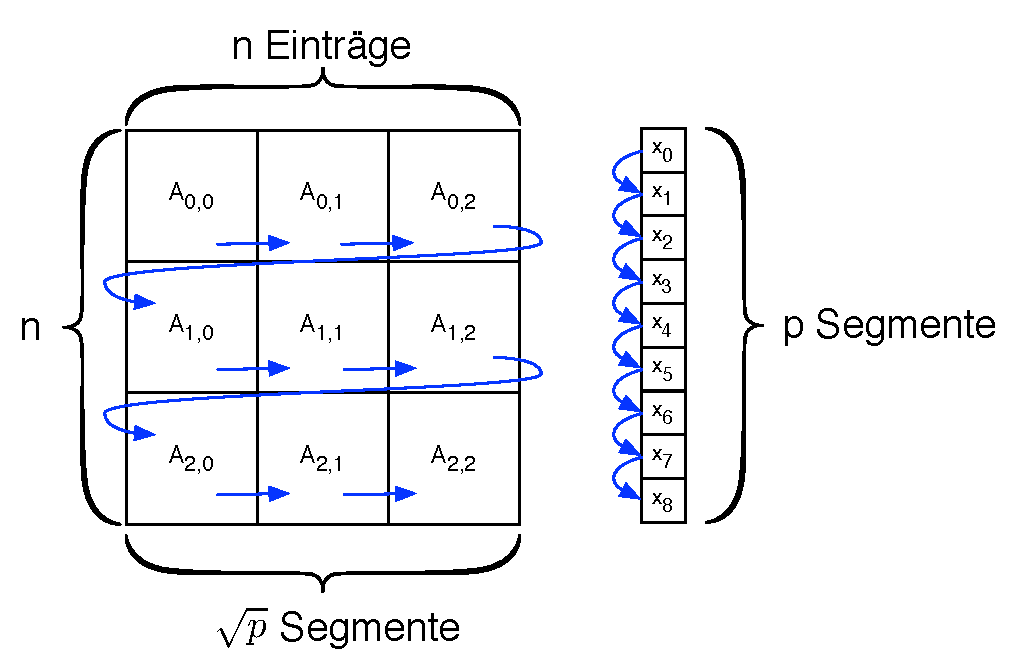
\includegraphics{pics/2d-decomposition.pdf}
	\caption{Der hier gezeigte quadratische Fall ist ein Spezialfall. n ist die Anzahl der Knoten, p die Anzahl der Places. In diesem Beispiel gibt es 9 Places. Dadurch, dass die Anzahl der Places eine Quadratzahl ist, ergibt sich horizontal und vertikal die selbe Zerlegung. Der Place mit der Nummer 0 speichert $A_{0,0}$ und $x_0$. Die blauen Pfeile zeigen, in welcher Reihenfolge die Daten auf die nachfolgenden Places aufgeteilt werden. Auf dem zweiten Place liegen demnach $A_{0,1}$ und $X_1$.}
\end{figure}

Auch bei der 2D Partitionierung müssen Vektoren auf die einzelnen Prozesse aufgeteilt werden. Angenommen die Adjazenzmatrix sei horizontal in h und vertikal in v Abschnitte unterteilt, außerdem sei n (Anzahl an Kanten) restlos durch p (Anzahl an Places) teilbar. Es gilt $h*v=p$. Die Menge der Places, die in der ersten Zeile der Unterteilung sind, besitzt dann den Abschnitt $ \left[1,n\right] * \left[1,\frac{n}{h}\right]$ der Adjazenzmatrix. Jedes Teilstück eines Vektors, den ein Place besitzt, ist  $l = \frac{1}{v} * \frac{n}{h} = \frac{n}{p}$ groß. Dadurch ist sichergestellt, dass das Teilstück eines Vektors, das der ersten Reihe gemeinsam gehört($\left[1,\frac{n}{p}\right] \cup \left[\frac{n}{p}+1,\frac{2n}{p}\right] \cup \dots \cup \left[\frac{(v-1)n}{p}+1,\frac{vn}{p}=\frac{n}{h}\right] $), dem horizontalen Teilstück $\left[1,\frac{n}{h}\right]$ des Matrixabschnittes entspricht, das genau dieser Reihe gehört.


Bei der zweidimensionalen Unterteilung wird der Breitensuch-Algorithmus als Folge von Matrix-Vektor-Operationen betrachtet, die dann einzeln parallelisiert werden. Angenommen der Algorithmus läuft auf nur einem Core, dann kann die Kommunikation und die Synchronisation eingespart werden. Der Pseudocode \ref{alg:2d_serial} beschreibt für diesen Fall die Essenz des Algorithmus. Der Algorithmus führt Iterationen aus, bis $x_k$ nur noch Nullen enthält: 
$$
x_{k+1} = \underbrace{ (A^T * x_k) }_{ \begin{tabular}{c} =1 an Stelle p \\ wenn Knoten p \\ von einem Knoten aus \\ $x_k$ erreichbar ist \end{tabular}} * \underbrace{\neg\sum_{i=1}^k x_i}_{\begin{tabular}{c} =1 an Stelle p, wenn \\ p noch unerreicht\end{tabular}}
$$ 
Das Produkt aus den beiden Vektoren entspricht der komponentenweisen Konjunktion der booleschen Werte. Die Matrixmultiplikation alleine reicht nicht aus, da Knoten sonst doppelt als erreicht markiert würden und somit eine falsche, zu große Distanz ausgegeben werden könnte. Es ist zu beachten, dass im Pseudocode die BFS-Distanz nicht gespeichert wird. Die BFS-Distanz kann aber leicht über die Nummer der Iteration herausgefunden und gesetzt werden. 

\begin{algorithm}[ht]
	\caption{BFS auf einem Place}
	\label{alg:2d_serial}
	\begin{algorithmic}[1]
		\State $f(s) \gets true$
		\State $t \gets 0^n$ // Nullvektor
		\While{$f \neq 0^n$}
			\State $x \gets A^T * f$
			\State $f \gets x * \neg t$
			\State $t \gets t + f$
		\EndWhile
	\end{algorithmic}
\end{algorithm}

Um den Code von Algorithmus \ref{alg:2d_serial} auf mehrere Places zu parallelisieren, werden die einzelnen Schritte betrachtet und die Daten entsprechend ausgetauscht. Die Zeilen 5 und 6 sind einfache eine komponentenweise Operationen und können daher lokal auf jedem Place stattfinden. In Zeile 4 wird die Matrix in der transponierten Form verwendet. Da der Algorithmus nie die nicht transponierte Form der Matrix nutzt, wird in Zukunft mit A die bereits transponierte Matrix bezeichnet. Um Zeile 4 zu parallelisieren ist einiger Aufwand notwendig. Um x[k] zu berechnen, muss sowohl die gesamte k-te Zeile aus A, als auch der gesamte Vektor f bekannt sein. Jeder Place besitzt aber nur einen Teil beider Datenstrukturen.



 Der Algorithmus wird dazu wieder in Phasen zerteilt, die in \ref{alg:2d_parallel} zu sehen sind.

 \begin{algorithm}[h]
	\caption{1D-partitionierte Breitensuche}
	\label{alg:2d_parallel}
	\begin{algorithmic}[1]
		\State {Startknoten: s, Kantenanzahl: n, Anzahl Places: p}
		\State bfsDistance : DistArray of size n \Comment{Mit $\infty$ initialisiert, 0 an Stelle s}
		\For{each place, do async on place}
			\State // Place an Position i,j im Grid
			\While{$f \neq 0$}
				\State{//Phase 1: Transpose f}
				\For{$ \mathit{node} \in \text{local part of f}$} 
					\State $j \gets \mathit{node} / \mathit{colsize} $
					\State put node in sendbuffer for column j
				\EndFor
				\State{//Phase 2: Kommunikation}
				\State{$\mathit{fTransposed} \gets \sum_{\textnormal{places in row j}}\mathit{sendbuffer}$}
				\State{$barriere$}

				\State{//Phase 3: Lokale Matrixmultiplikation}
				\For{$i=rowFrom \to rowTo$}
					\State $t[i] \gets A\big|_{i-th\;row} \cdot \mathit{fTransposed}$
				\EndFor

				\State{//Phase 4: Ergebnisse der Reihe zusammenführen}
				\For{$node \in t$}
					\State{Send node to owners \textit{t}-vector}
				\EndFor

				\State{$barriere$}
				\State{//Phase 5: Lokale updates durchführen}
				\State $f \gets t * (d==\infty)$
				\State Set d[i] = iteration number, where f[i]=true
			\EndWhile
		\EndFor
	\end{algorithmic}
\end{algorithm}
Für die folgenden Erläuterungen wird angenommen, dass es n Knoten gibt und die Adjazenzmatrix ($n \times n$) auf $g^2$ Places aufgeteilt ist, also in der Vertikalen und der Horizontalen je g Unterteilungen stattfanden. Der Place p besitze den Ausschnitt der Matrix $\left[x_{von}, x_{bis} \right] \times \left[y_{von}, y_{bis} \right]$. Dieser Ausschnitt sei der i-ten Reihe von oben und der j-te Spalte von links. 


\subsection{Phase 1: Transponieren des Vektors f} % (fold)
\label{sub:transponieren_des_vektors_f}
Es soll berechnet werden, ob Knoten k im nächsten Iterationsschritt erreicht werden kann. Dazu sei $k \in \left[y_{von}, y_{bis} \right]$. Daraus folgt, dass Place P einen Teil der Adjazenzmatix besitzt, der nötig ist, um festzustellen, ob k erreicht werden kann. Place p weiß allerdings nur, ob k von einem Knoten zwischen $x_{von}$ und $x_{bis}$ erreichbar ist. Um für diese Iteration ein Ergebnis zu berechnen, braucht er also die Information, welche dieser Knoten im Intervall $\left[x_{von}, x_{bis} \right]$ aktuell aktive Knoten sind. Diese Information ist aber aufgeteilt auf alle Places in der j-ten Reihe der Unterteilung. Für die Berechnung benötigt aber jeder der Places in der j-ten Spalte (also unter anderem Place p) genau diese Information. Deswegen wird die erste Phase als Transponieren bezeichnet. Der Algorithmus iteriert auf jedem Place über alle aktiven Knoten und berechnet, welche Spalte der Dekomposition der Matrix wissen muss, dass dieser Knoten aktiv ist. Die Formel kann beispielsweise so aussehen: $$\mathit{Spaltennummer}= \lfloor\frac{\mathit{Knotennummer}}{\mathit{Spaltenbreite}}\rfloor$$
% subsection transponieren_des_vektors_f (end)

\subsection{Phase 2: Kommunikation} % (fold)
\label{ssub:kommunikation}
Nachdem die Knoten sortiert sind, werden sie jeweils nebenläufig an den berechneten Empfänger geschickt. In der Implementierung zu dieser Arbeit steht dazu auf jedem Empfänger eine Empfangspuffer bereit. Die Verwendung eines einzelnen Empfangspuffers bedeutet, dass sich alle Sender synchronisieren müssen. Der Aufwand ist aber vernachlässigbar, verglichen mit dem Aufwand der Kommunikation. In einer optimierten Variante könnte auf jedem Place für jeden Sender ein eigener Empfangspuffer verfügbar sein, wodurch die Synchronisation wegfallen würde.
% subsection kommunikation (end)

\subsection{Phase 3: Lokale Matrixmultiplikation} % (fold)
\label{ssub:lokale_matrixmultiplikation}
Bevor dieser Schritt stattfindet, muss sichergestellt werden, dass der vorherige Schritt vollständig abgeschlossen ist. Dazu wird eine globale Barriere über alle Places verwendet. Die Matrixdatenstruktur sieht so aus, dass ein Place zu jedem Knoten in $\left[x_{von}, x_{bis} \right]$ eine Liste aller Knoten hält, die von diesem Knoten aus erreichbar sind. Es wird über alle aktiven Knoten iteriert und die Listen der erreichbaren Knoten aller aktiven Knoten aneinander gehängt. Diese Liste enthält Knoten, die in der nächsten Iteration aktiv sind, falls sie nicht schon aktiv waren. Es ist zu beachten, dass jeder Knoten in dieser Liste in dem Intervall $\left[y_{von}, y_{bis} \right]$ liegt und dass jeder Place, der ebenfalls in der i-ten Reihe ist, ein Liste von aktiven Knoten hält, die in genau demselben Intervall sind. Nur eine Reihe gemeinsam weiß exakt, welche Knoten aktiv sein werden und welche nicht.
% subsection lokale_matrixmultiplikation (end)

\subsection{Phase 4: Ergebnisse der Reihe zusammenführen} % (fold)
\label{ssub:ergebnisse_der_reihe_zusammenf_hren}
Nach dem vorherigen Schritt weiß jeder Place von einigen Knoten, dass dieser erreicht wurden. Je eine Reihe gemeinsam hat die Information, welcher von den $n/h$ Knoten, die ihnen gemeinsam gehören, erreicht wurden. Wie oben bei der Vektordekomposition zu sehen, ist jeder Knoten genau einem Place zugeordnet. Die folgende Kommunikation passiert nur zwischen Places einer Reihe, da der Abschnitt des Distanzvektors, der dieser Reihe gemeinsam gehört, genau dem Abschnitt $\left[y_{von}, y_{bis} \right]$ entspricht. Das bedeutet, dass alle Knoten, die in einer Reihe der Dekomposition stehen, untereinander austauschen müssen, welche Knoten erreicht wurde. Die Place-Nummer des Besitzers eines Knotens ist $\mathit{Placenummer}=\lfloor\frac{\mathit{Knotennummer}}{\mathit{Anzahl Places}}\rfloor$. Jeder sendet an den Besitzer des Knotens, falls dieser Knoten aktiv ist, die Knotennummer. Wenn niemand dem Besitzer eines Knotens sendet, dass dieser erreicht wurde, ist der Knoten nicht erreicht worden. Es muss auf alle Sendevorgänge gewartet werden, bevor weitere Berechnungen stattfinden können. Deswegen ist nach dieser Phase eine globale Barriere von Nöten.
% subsection ergebnisse_der_reihe_zusammenf_hren (end)

\subsection{Phase 5: Lokale Aktualisierungen durchführen} % (fold)
\label{ssub:lokale_updates_durchf_hren}
Die letzte Phase entspricht der Aktualisierung der BFS-Distanzen der konventionellen Breitensuche. Es liegt eine Liste der in dieser Iteration erreichten Knoten vor. Zu jedem Knoten ist bekannt, ob er bereits erreicht wurde oder nicht. Falls nicht, wird die BFS-Distanz auf die Nummer der aktuellen Iteration gesetzt.
% subsection lokale_updates_durchf_hren (end)
% section 2d_partitionierung (end)

\section{Allreduce} % (fold)
\label{sub:allreduce}
Ein Detail wichtiges Detail, dass bisher noch keine Erwähnung fand, findet sich sowohl in Algorithmus \ref{alg:1d_bfs_abstract} als auch in Algorithmus \ref{alg:2d_parallel} in Zeile 5. Beide Zeilen bedeuten: \textit{solange es mindestens einen aktiven Knoten gibt, iteriere...} Es gibt genau dann noch aktive Knoten, wenn mindestens ein Place mindestens einen aktiven Knoten hat. Es dürfen aber alle Prozesse auf allen Places erst dann aufhören zu iterieren, wenn auf keinem Place mehr ein aktiver Knoten vorhanden ist. In boolesches Logik ausgedrückt, muss jeder Prozess der Allgemeinheit mitteilen, ob er noch aktive Knoten hat. Diese Information muss mittels ODER verknüpft werden. Das Ergebnis der Verkñupfung muss allen Prozessen mitgeteilt werden. Diesen Vorgang nennt man an MPI angelehnt Allreduce. Es wurde die Implementierung aus der der X10 Standard Library benutzt. Falls X10 zum Beispiel über MPI kommuniziert, ist es unter Umständen wesentlich schneller, die Allreduce Operation aus einer MPI Hardware zu nutzen, als die selbe Funktionalität nachzuprogrammieren.  
% section allreduce (end)

\section{Optimierungen} % (fold)
\label{sec:optimierungen}
Auch bei der Dekomposition in zwei Dimensionen gibt es zu beachten, dass die Listen, die in Phase 3 erstellt und in Phase 4 versendet werden, Duplikate enthalten können. Um so dichter ein Graph ist, um so wichtiger ist es, diese Listen frei von Duplikaten zu machen. Siehe dazu Abschnitt \ref{sub:duplikate_in_sendepuffern}. Ohne weitere Abwandlungen kann auch die Optimierung \ref{ssub:zusammenlegung_der_ersten_und_letzten_phase} angewandt werden. Je nach gewählter Datenstruktur können auch die Adjazenzlisten wie in \ref{ssub:adjazenslisten_löschen} gelöscht werden, was bei der Implementierung zu dieser Arbeit gemacht wurde. 
% section optimierungen (end)
% chapter paralleler_algorithmus (end)